\documentclass[11pt,fleqn,a4paper,]{LegrandOrangeBook}
\addbibresource{sample.bib} % Bibliography file
\definecolor{ocre}{RGB}{243, 102, 25} 
\chapterimage{orange1.jpg} 
\chapterspaceabove{6.5cm}
\chapterspacebelow{6.75cm} 
%\begin{theorem}[Name of the theorem]
%\begin{exercise}
%\begin{example}[Example name]
%\begin{definition}[Definition name]
%\begin{corollary}[Corollary name]
%\begin{remark}
%\begin{proposition}[Proposition name]
%\begin{problem}
%\begin{vocabulary}[Word]
%----------------------------------------------------------------------------------------
\begin{document}
%----------------------------------------------------------------------------------------
\section{Mediciones de radiofrecuencia}
\subsection{¿Qué es radio enlace?}
El Radio Enlace o radioenlace punto a punto, es un sistema de conexiones entre dos o más terminales (antenas) que utilizan ondas electromagnéticas para transmitir datos, ya sea para dar servicios de operador VoIP, servicios de telefonía móvil para empresas, Internet, etc.\\
El equipo terminal esta compuesto por: antena, alimentador, radio y multiplexor. Los sistemas de radio de basan en el envío de ondas electromagnéticas a través del espacio libre para poder unir un equipo terminal con otro equipo terminal.\\
El radio digital convierte el tren de pulsos en una señal modulada en PSK en alta frecuencia:
El radio esta compuesto de modulador ,transmisor, receptor y demodulador. Dos radio digitales con antenas que se miran forman un radioenlace.
\begin{table}[H]
\begin{tabular}{|l|l|l|l|l|l|}
\hline
\rowcolor[HTML]{68CBD0} 
Banda & Mux & Velocidad de bits & Modulación & Alimentador  & Antenna         \\ \hline
VHF   & 2   & 64-128 kbit/s     & PSK        & Coaxial      & Yagui           \\ \hline
UHF   & 30  & 2 MBit/s          & 4-PSK      & Coaxial      & Semi-parabolica \\ \hline
SHF   & PDH & 8, 34, 140 Mbit/s & 16-QAM     & Guía de onda & Parabólica      \\ \hline
SHF   & SDH & 565 Mbit/s        & 128-QAM    & Guía de onda & Parabólica      \\ \hline
\end{tabular}
\caption{Bandas de radio enlace digital}
\end{table}
\subsection{Bandas de frecuencia}
Las señales eléctricas que contienen información se transmiten a través de una determinada distancia empleando una diversidad de medios de transmisión tales como par de alambres, cable multipar, cable coaxial, cable UTP, Sistemas de Radio y Fibras ópticas. Una señal eléctrica es una forma de onda electromagnética caracterizada por una determinada frecuencia y longitud de onda que se encuentra dentro de una banda frecuencia del espectro electromagnético y para cada banda se necesita utilizar un medio de transmisión adecuado.
% Please add the following required packages to your document preamble:
% \usepackage[table,xcdraw]{xcolor}
% If you use beamer only pass "xcolor=table" option, i.e. \documentclass[xcolor=table]{beamer}
\begin{table}[H]
\begin{tabular}{|m{0.15\linewidth}|m{0.15\linewidth}|m{0.3\linewidth}|m{0.4\linewidth}|}
\hline
\rowcolor[HTML]{F8FF00} 
\begin{tabular}[c]{@{}l@{}}Medio de\\ transmisión\end{tabular}                                                                                & \begin{tabular}[c]{@{}l@{}}Longitud\\ de Onda\end{tabular} & \begin{tabular}[c]{@{}l@{}}Banda de\\ frecuencia\end{tabular}                                           & Aplicaciones                                                                                                                                                                                                                                                          \\ \hline
Fibras ópticas                                                                                                                                & 3-0.3$\mu$m                                                & \begin{tabular}[c]{@{}l@{}}Ultravioleta\\ Luz visible\\ Infrarojo\\ $10^2-10^3$ THz\end{tabular}        & \begin{tabular}[c]{@{}l@{}}Telefonia de muy alta capacidad.\\ Servicios de banda ancha\\(SONET, SDH y ATM),\\Video conferencia, CATV por F. O.\end{tabular}                                                                                                            \\ \hline
\begin{tabular}[c]{@{}l@{}}Guías de onda\\de línea visual\end{tabular}                                                                     & 1-0.1 cm                                                   & \begin{tabular}[c]{@{}l@{}}30-300 GHz\\ Extremadamente\\ Alta frecuencia (EHF)\end{tabular}             & \begin{tabular}[c]{@{}l@{}}Comuniaciones militar por satelite,\\radioastronomia\\sistemas de aterrizaje\\por radar.\end{tabular}                                                                                                                                      \\ \hline
{\color[HTML]{34FF34} \begin{tabular}[c]{@{}l@{}}Guías de onda\\de línea visual\end{tabular}}                                              & {\color[HTML]{34FF34} 10-1 cm}                             & {\color[HTML]{34FF34} \begin{tabular}[c]{@{}l@{}}3-30 GHz\\ Super alta frec.\\ (SHF)\end{tabular}}      & {\color[HTML]{34FF34} \begin{tabular}[c]{@{}l@{}}Comunicaciones vía satelite,\\radio microonda análogico,\\radio microonda digital\\y sistema de operación\\aérea por radar.\end{tabular}}                                                                              \\ \hline
{\color[HTML]{3531FF} Onda directa}                                                                                                           & {\color[HTML]{3531FF} 100-10 cm}                           & {\color[HTML]{3531FF} \begin{tabular}[c]{@{}l@{}}0.3-3 GHz\\ Ultra alta frec.\\ (UHF)\end{tabular}}     & {\color[HTML]{3531FF} \begin{tabular}[c]{@{}l@{}}Video Difusión (UHF),\\telemetría por radar,\\comunicación militar por\\satélite, multiacceso radial\\UHF, radio PCM,  multiacceso\\digital, telefonía celular,\\radio digital de espectro\\ensanchado\end{tabular}} \\ \hline
{\color[HTML]{FE0000} \begin{tabular}[c]{@{}l@{}}Cable coaxial\\ cable UTP\\(CAT5) Onda directa\end{tabular}}                                & {\color[HTML]{FE0000} 10-1 m}                              & {\color[HTML]{FE0000} \begin{tabular}[c]{@{}l@{}}30-300 MHz\\ Muy alta frecuencia\\ (VHF)\end{tabular}} & {\color[HTML]{FE0000} \begin{tabular}[c]{@{}l@{}}Video difusión (VHF), radio difusión\\FM, multiacceso radial\\VHF, sistema CATV,\\radio monocanal y radio\\enlace para cursar voz-datos.\end{tabular}}                                                                 \\ \hline
\begin{tabular}[c]{@{}l@{}}Cable coaxial,\\cable UTP\\(CAT 3), cable\\UTP (CAT 4),\\onda de cielo\\(reflexión de\\la ionosfera)\end{tabular} & 100-10 m                                                   & \begin{tabular}[c]{@{}l@{}}3-30Mhz\\ Alta frecuencia\\ (HF)\end{tabular}                                & \begin{tabular}[c]{@{}l@{}}Radio aficionados, comunicaciones\\militares,radio telefonía móvil,\\y comunicación marítima.\end{tabular}                                                                                                                                \\ \hline
\end{tabular}
\end{table}
\begin{exercise}[Generador de audio]
Dado un generador de audio calibrado en 0dBm a 600$\Omega$, 1kHz.
\begin{center}
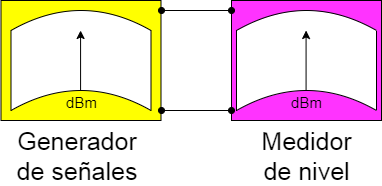
\includegraphics[scale=0.5]{IM/IM1.png}
\end{center}
Calcular:\\
\begin{enumerate}
\item Determinar en mV, la señal que se recibe en un medidor de nivel si la
medida es hecha a 600 $\Omega$.
\item Determinar en mV, la señal que se recibe en un medidor de nivel si la
medida es hecha a 75 $\Omega$.
\end{enumerate}
\textbf{Solución:}\\
Para el primer punto, nos esta ofreciendo el dato en \textbf{dBm}, usando la eq. \ref{art:dbm} pero ten en cuenta que sabemos que es 0dBm, no nos esta dando la potencia. Planteamos:
\begin{align*}
0dBm&=10\cdot\log_{10}\left(\frac{P_{out}}{1mW}\right)dBm\\
0dBm&=\cdot\log_{10}\left(\frac{P_{out}}{1mW}\right)dBm\\
0&=\log_{10}\left(\frac{P_{out}mW}{1mW}\right)\\
10^0&=\frac{P_{out}}{1mW}\\
P_{out}&=1mW\simeq 10^{-3}W
\end{align*}
Ya tenemos la potencia de salida en watts, nos pide la señal que recibe el medidor con una resistencia de 600$\Omega$, usando la ecuación de potencia \ref{eq:potencia}:
\begin{align*}
V=&\sqrt{P\cdot R}\\
V=&\sqrt{10^{-3}\cdot 600\Omega}
\end{align*}
\begin{equation*}
\boxed{V=0.7745V\simeq 774.5mV}
\end{equation*}
Este proceso resulto fácil pues la medida es hecha a 600$\Omega$, y pues nuestro circuito ya esta hecho para esa resistencia.\\
\textbf{El punto 2} nos habla de otra carga a 75$\Omega$. Para ello usaremos el dato del inciso 1 para obtener al valor de la fuente del generador:
\begin{center}
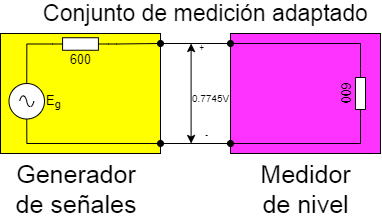
\includegraphics[scale=0.5]{IM/IM2.png}
\end{center}
El valor hallado en el punto 1 es el valor de entrada para el medidor, usando un divisor de voltaje:
\begin{align*}
0.7785=&\frac{E_g\cdot 600}{600+600}\\
E_g=&1.549V
\end{align*}
Bien, ya hallamos el voltaje de la fuente. Ahora tenemos lo datos para cambiar la carga de 600$\Omega$ por 75 $\Omega$ en el medidor de nivel:
\begin{center}
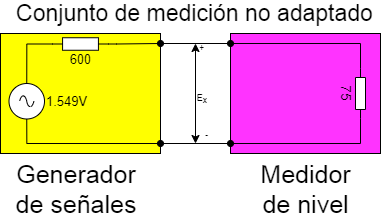
\includegraphics[scale=0.5]{IM/IM3.png}
\end{center}
Nuevamente, usando un dividor de voltaje:
\begin{align*}
E_x&=\frac{1.54\cdot 75}{600+75}
\end{align*}
\begin{equation*}
\boxed{E_x=0.1721V}
\end{equation*}
Calculando la potencia de salida del generador para un medidor desadaptado:
\begin{align*}
P_x&=\frac{0.1721^2}{75}\\
P_x&=0.394 mW
\end{align*}
Expresando $P_x$ en dBm:
\begin{align*}
L_{P/1mW}&=10\cdot \log_{10}\left(\frac{0.394mW}{1mW}\right)dBm\\
L_{P/1mW}&=-4.04dBm
\end{align*}
Analizamos las respuestas como: Si tenemos un generador a 600$\Omega$ con lineas de transmisión a 600$\Omega$ y medidor a 600$\Omega$, si yo generó 0dBm en el generador, al medidor me llegará 0dBm: calibración exitosa, pero si cambiamos tan solo el receptor a 75$\Omega$, no me va llegar los 0dBm generados, sino me llegará aproximadamente los -4.04dBm, cosa que esta mal.
\end{exercise}
\begin{definition}[Potencia Isotrópica Radiada Equivalente]
Cantidad de potencia que emitiría una antena isotrópica teórica para producir la densidad de potencia observada en la dirección de máxima ganancia de una antena.\\
Definida como:
\begin{equation}
\label{eq:Pire}
P_{IRE}=P_t-L_c+G_a
\end{equation}
Donde:\\
\begin{itemize}
\item $P_t$: Potencia del transmisor.(dBm)
\item $L_c$: Perdidas de cable.(dB)
\item $G_a$: Ganancia de la antena. (dBi, relativo a la antena de referencia isotrópica)
\end{itemize}
\end{definition}
\begin{exercise}
Se tiene un transmisor de 100 WATTS que opera en la banda HF, con cable coaxial de atenuación de 1,7 dB/100m y una antena de ganancia de 10 dBi. Calcular la potencia radiada efectiva.\\
\begin{center}
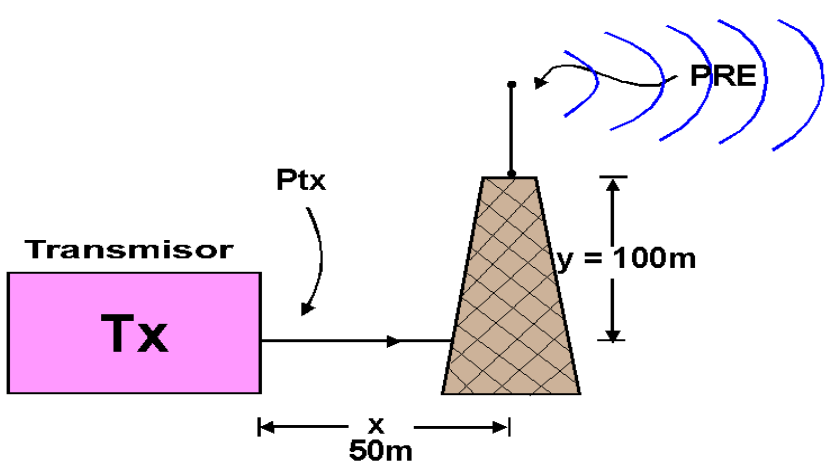
\includegraphics[scale=0.5]{IM/IM4.png}
\end{center}
\textbf{Solución}:
Usando la ecuación \ref{eq:Pire}, debemos acomodar nuestros datos. Empezamos con el calculo de $P_{tx}$=100W:
\begin{align*}
L_{P/1mW}&=10\cdot \log_{10}\left(\frac{100\times ^3mW}{1mW}\right)dBm\\
L_{P/1mW}&=50dBm
\end{align*}
El \textbf{calculo por perdida en el cable}, vemos que el total de cable es de 150m: 50 desde el transmisor a la antena y 100m de altura de la antena:
\begin{align*}
L_c&=150m\times\frac{1.7dB}{100m}\\
L_c&=2.55dB
\end{align*}
Reemplazando los datos obtenidos en \ref{eq:Pire}:
\begin{align*}
P_{IRE}&=50-2.55+10\\
P_{IRE}&=54.45 dBm
\end{align*}
Podemos pasar de dBm a Watts:
\begin{align*}
57.45dBm&=10\cdot \log_{10}\left(\frac{P_{IRE}mW}{1mW}\right)dBm\\
P_{IRE}&=555.9 W
\end{align*}
\end{exercise}
\begin{exercise}[Atenuadores]
Se tiene un transmisor en la banda UHF con una salida de potencia RF de 27 dBm. Encontrar la configuración de atenuadores adecuada para que
pueda ser medido con un Watímetro de rango 0 a -15dBm y no dañe el instrumento.\\
\begin{center}
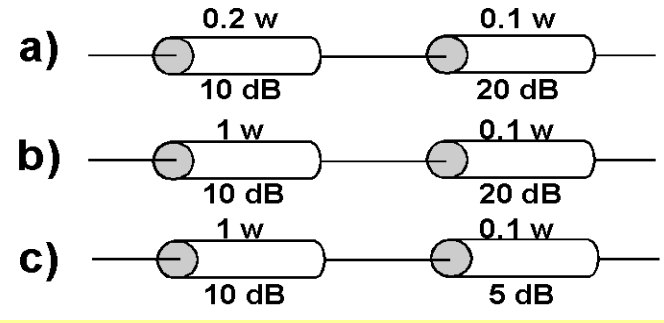
\includegraphics[scale=0.5]{IM/IM5.png}
\end{center}
\begin{center}
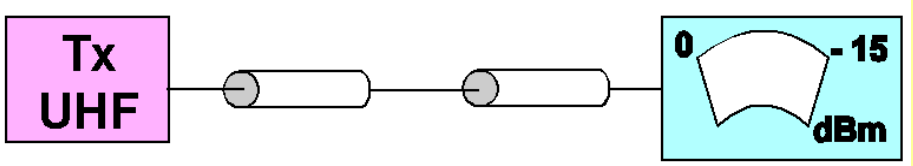
\includegraphics[scale=0.5]{IM/IM6.png}
\end{center}
\textbf{Solución:}\\
Antes de seguir, vamos a recalcar que es un \textbf{atenuador}, vamos a calcular los niveles a través de cada atenuado para cada opción. La salida del transmisor es de 27dBm, para cada opción restamos el valor de cada atenuador:
\begin{center}
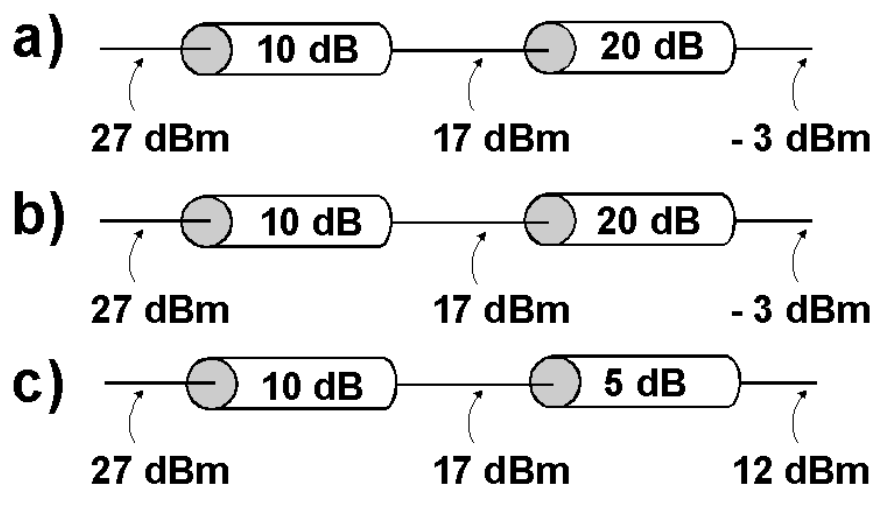
\includegraphics[scale=0.35]{IM/IM7.png}
\end{center}
Se descarta la opcion C ya que el nivel final antes de entrar al vatímetro es de 12 dBm, estando fuera del rango de 0 a -15 dBm del vatímetro y en consecuencia puede dañar el instrumento. Aún nos quedan dos opciones, ahora debemos de analizar a nivel de potencia. Analicemos la opción a nivel de \textbf{potencia}:
\begin{align*}
27=&10\cdot \log_{10}\left(\frac{P_{out}mW}{1mW}\right)dBm\\
P_{out}&=0.5W
\end{align*}
Ya salida en watts del transmisor es de 0.5W pero vemos que su primer atenuador solo resiste 0.2W, por lo tanto no es adecuado. Descartando así la opción a. Probamos la opción b si es correcta o incorrecta, ojo, analizamos el segundo atenuador de la opción b, pues el primer atenuador resiste 1W, así que no habrá problema:
\begin{align*}
17=&10\cdot \log_{10}\left(\frac{P_{out}mW}{1mW}\right)dBm\\
P_{out}&=0.005W
\end{align*}
La potencia es de 0.005W cuando el segundo atenuador puede aguantar 0.1W y no habrá problema, así que la opción correcta es la b.
\end{exercise}
\begin{example}
Es un sistema de recepción TV satélite, la unidad interna tiene una impedancia de entrada de 50 W y el fabricante indica en su catalogo que
el nivel de señal mínimo de entrada es de - 60 dBm.
\begin{itemize}
\item Cual es el nivel en $\mu$V. Rpta: 223.6$\mu$V
\item Cual es el nivel en dB$\mu$V. Rpta: 46.98dB$\mu$V
\item Cual es la Potencia mW: Rpta: 1mW
\end{itemize}
\end{example}
\begin{example}

\end{example}
%\section{Capa física en redes de datos}
%\section{Protocolos estándares y propietarios}
%\section{Capa de enlace y la evolución de las telecomunicaciones}
%----------------------------------------------------------------------------------------
\end{document}
%----------------------------------------------------------------------------------------
